\documentclass[twoside]{dlu-thesis}


\usepackage{listings}
\usepackage{varwidth}  % 提供varwidth环境
\usepackage{calc}      % 用于长度计算


\lstdefinestyle{lfonts}{
    basicstyle   = \footnotesize\ttfamily,
    stringstyle  = \color{purple},
    keywordstyle = \color{blue!60!black}\bfseries,
    commentstyle = \color{olive},
}

\lstdefinestyle{lnumbers}{
    numbers     = left,
    numberstyle = \tiny,
    numbersep   = 1em,
    firstnumber = 1,
    stepnumber  = 1,
}

\lstdefinestyle{llayout}{
    breaklines = true,
    tabsize    = 2,
    % columns    = flexible,
}

\lstdefinestyle{lgeometry}{
    xleftmargin  = 20pt,
    xrightmargin = 0pt,
    frame        = tb,
    framesep     = \fboxsep,
    framexleftmargin = 20pt,
}

\lstdefinestyle{lstrings}{
    showstringspaces = false,
}

\lstdefinestyle{lgeneral}{
    style = lfonts,
    style = lnumbers,
    style = llayout,
    style = lgeometry,
    style = lstrings,
}

\lstdefinestyle{TeX}{
    language = {tex},
    style    = lgeneral,
}

% chapters/info.tex (使用 \newcommand)

\newcommand{\ClassificationNumber}{}
\newcommand{\Secretlevel}{}
\newcommand{\UDC}{}
\newcommand{\No}{}

\newcommand{\myThesisTitle}{我的论文中文标题}
\newcommand{\mysubTitle}{题目太长了}
\newcommand{\myAuthorName}{我的名字}
\newcommand{\mygrade}{研三}
\newcommand{\mySupervisorName}{导师名字}
\newcommand{\myMajorName}{我的专业}
\newcommand{\myDefenseDate}{2024-07-25}



\newcommand{\myThesisTitleEN}{My Thesis English Title} % 单独定义英文标题
\newcommand{\myAuthorNameEN}{My English name}
\newcommand{\mySupervisorNameEN}{Supervisor English name}
\newcommand{\myMajorNameEN}{MyMajorNameEN}
\newcommand{\myDefenceChairman}{MyDefenceChairman}
 % 在导言区包含信息定义文件

\begin{document}
%-----------------------------------------------------------------------------------------------------------------------


\pagestyle{empty} % 设置封面和声明页为无页眉页脚样式
    % preface/cover.tex - 设计封面,使用 \newcommand 定义的命令

\begin{titlepage}
    \centering
    \renewcommand{\baselinestretch}{1.0}\normalsize

    % --- 页眉左右角信息 ---
    %\vspace*{3.5cm}
    \begin{minipage}[t]{0.45\textwidth}
        \raggedright \zihao{-4} \linespread{1.5}\selectfont
        \makebox[3em][l]{\textbf{分类号}} \underline{\makebox[3cm]{\hfill\raisebox{0.5ex}{\textbf{\ClassificationNumber}}\hfill}} \\
        \makebox[3em][l]{\textbf{UDC}} \underline{\makebox[3cm]{\hfill\raisebox{0.5ex}{\textbf{\UDC}}\hfill}}
    \end{minipage}%
    \hspace{0.05\textwidth}%
    \begin{minipage}[t]{0.45\textwidth}
        \raggedleft \zihao{-4} \linespread{1.5}\selectfont  % 设置1.5倍行距
        \makebox[3em][l]{\textbf{密级}} \underline{\makebox[3cm]{\hfill\raisebox{0.5ex}{\textbf{\Secretlevel}}\hfill}} \\
        \makebox[3em][l]{\textbf{编号}} \underline{\makebox[3cm]{\hfill\raisebox{0.5ex}{\textbf{\No}}\hfill}}
    \end{minipage}

    % --- 学校和论文类型 ---
    \vspace{2cm}
    {\zihao{-1}\heiti\bfseries  大\hspace{0.8em}连\hspace{0.8em}大\hspace{0.8em}学} % 调用自定义命令
    \vskip 0.5cm
    {\zihao{-1}\zhongsong\bfseries 硕\hspace{0.8em}士\hspace{0.8em}学\hspace{0.8em}位\hspace{0.8em}论\hspace{0.8em}文} % 调用自定义命令
    \vfill

    \scalebox{1.0}{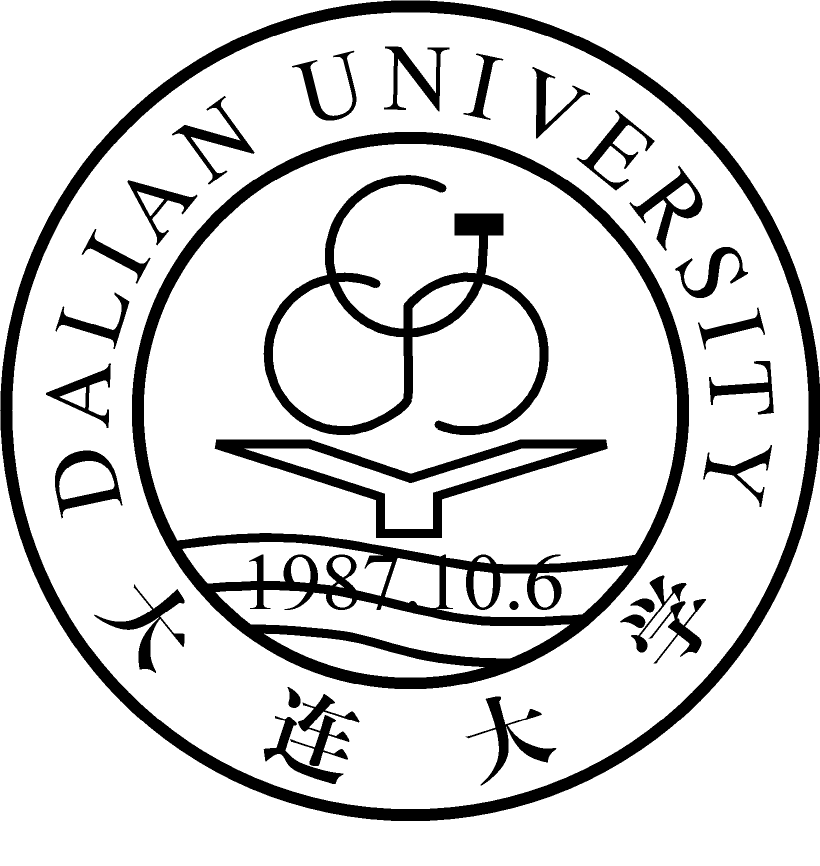
\includegraphics[width=4.87cm]{preface/logo.png}}

    % --- 论文标题 ---
    \vspace{2cm}
    {
      \raggedright  % 左对齐
      \heiti
      \fontsize{20}{24}\heiti
      \bfseries
      论\hspace{0.3em}文\hspace{0.3em}题\hspace{0.3em}目
      \underline{\makebox[11cm]{\hfill\raisebox{0.5ex}{\myThesisTitle}\hfill}} \\
      \vspace{10pt} % 下划线与副标题下划线之间的间距
      \hspace{3.2em} \underline{\makebox[11cm]{\hfill\raisebox{0.5ex}{\mysubTitle}\hfill}}
    }
    \vfill


    % --- 作者、导师等信息 ---  
\newcommand{\coverlength}{2.7cm}
\vskip 1.0cm 
\begin{center}
\renewcommand\arraystretch{2}
\begin{tabular}{l}
\makebox[\coverlength][s]{\zihao{4}\kaishu \bf 姓名}~~\\
\makebox[\coverlength][s]{\zihao{4}\kaishu \bf 学科、专业}\\ 
\makebox[\coverlength][s]{\zihao{4}\kaishu \bf 指导教师}\\
\makebox[\coverlength][s]{\zihao{4}\kaishu \bf 年级}\\ 
\makebox[\coverlength][s]{\zihao{4}\kaishu \bf 论文答辩日期}
\end{tabular}
\begin{tabular}{@{}>{\centering\arraybackslash}p{5cm}@{}}
{\zihao{4}\kaishu \bf  ~~\myAuthorName~~}\\ 
\hline {\zihao{4}\kaishu \bf ~~\myMajorName~~}\\ 
\hline {\zihao{4}\kaishu \bf ~~\mySupervisorName~~}\\ 
\hline {\zihao{4}\kaishu \bf  ~~\mygrade~~}\\
\hline{\zihao{4}\kaishu \bf ~~\myDefenseDate~~ }\\
\hline
\end{tabular}
\end{center}



%    \renewcommand{\baselinestretch}{\mybaselinestretch}\normalsize % 恢复行距
\end{titlepage}
\vfill % 填充剩余空间,避免自动分页
    % preface/cover-en.tex - 使用 info.tex 中定义的命令
\begin{titlepage}

    \centering % 居中页面内容
    \renewcommand{\baselinestretch}{1.0}\normalsize % 封面通常用单倍行距

    %\vspace*{2cm} % 顶部留白

    {\fontsize{20}{24}\bfseries Master's\hspace{0.5em}Degree\hspace{0.5em}Dissertation\par} % 顶部标题


\raggedright  % 左对齐

    \vspace{6cm}
    {
      \heiti
      \zihao{-1}
      \bfseries
      Title:\myThesisTitleEN
    }
    
    \vspace{5cm}
    
    % --- 底部信息块 ---
    \large
    \begin{tabular}{@{}ll@{}}
        \rule{0pt}{3ex}
        \textbf{M.S. candidate:} & \textbf{\myAuthorNameEN} \\ % <--- 使用英文作者名命令
        \rule{0pt}{3ex}
        \textbf{Advisor:} & \textbf{\mySupervisorNameEN} \\ % <--- 使用英文导师名命令
        \rule{0pt}{3ex}
        \textbf{Field of research:} & \textbf{\myMajorNameEN} \\ % <--- 使用英文专业名命令
        \rule{0pt}{3ex}
        \textbf{Date of defence:} & \textbf{\myDefenseDate} \\ % <--- 使用答辩日期命令
        \rule{0pt}{3ex}
        \textbf{Chairman of defence committee:} & \textbf{\myDefenceChairman} \\ % <--- 使用答辩主席命令 (定义在 main.tex 或 info.tex)
        \rule{0pt}{3ex}
        \textbf{Degree awarded by:} & \textbf{Dalian University} \\
    \end{tabular}

    \vspace*{3cm} % 底部留白
   % \renewcommand{\baselinestretch}{\mybaselinestretch}\normalsize % 恢复行距 (如果需要)


\vfill % 填充剩余空间,避免自动分页
\end{titlepage}
\cleardoublepage 

% 确保原创性声明 PDF 从奇数页开始

\includepdf[pages=-]{statement.pdf}
\cleardoublepage

\frontmatter
\pagestyle{dlu@headings}

% 先添加版权页到目录(此时还未生成目录)
%\cleardoublepage
%\phantomsection
%\addcontentsline{toc}{chapter}{版权声明}  % 先添加到目录
%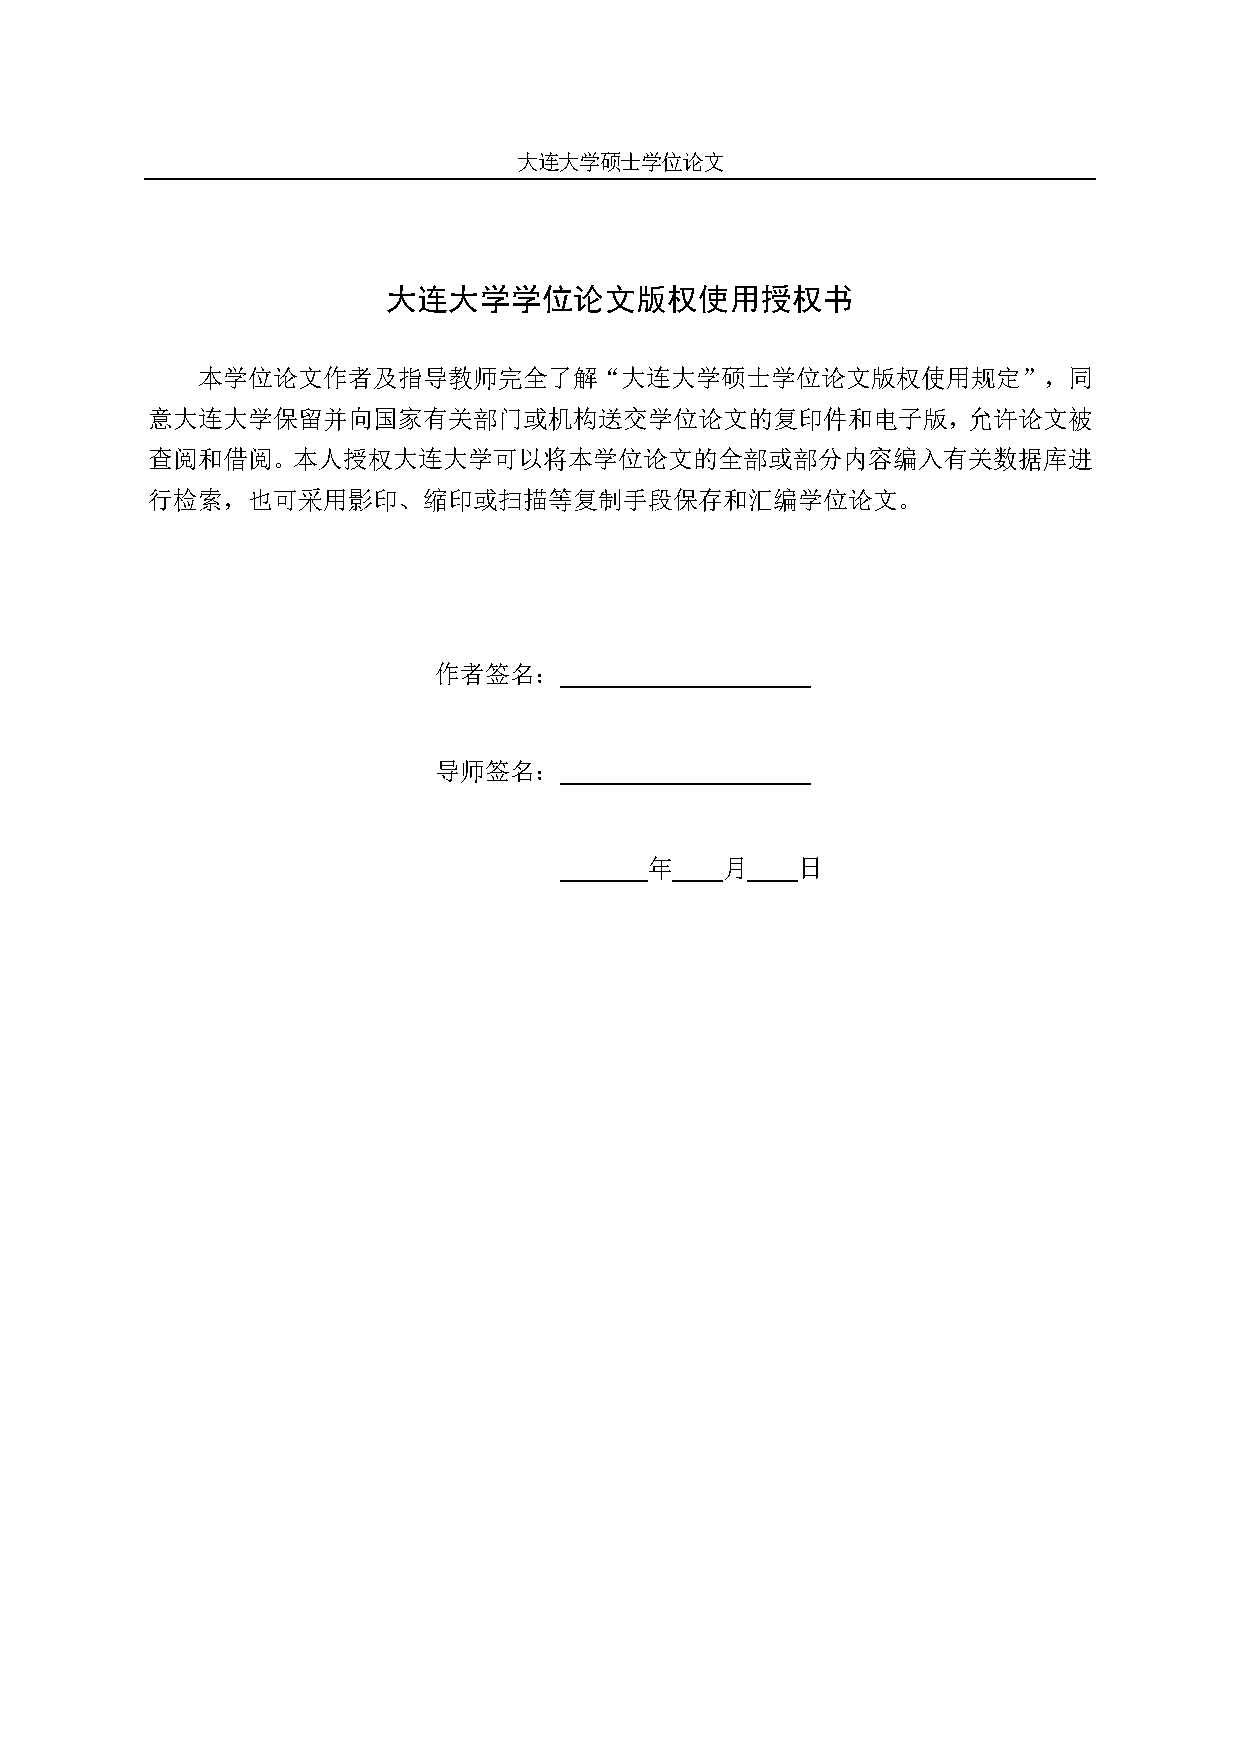
\includepdf[pages=-]{copyright.pdf}

\begin{abstract}

本文给出了大连大学硕士学位论文的写作规范和排版格式要求。文中格式可作为编排硕士学位论文的格式模板,供研究生参考使用。

摘要部分说明:

“摘要”是摘要部分的标题,不可省略。

标题“摘要”选用模板中的样式所定义的“标题1”,再居中;或者手动设置成字体:黑体,居中,字号:小三,1.5倍行距,段后11磅,段前为0。

论文摘要是学位论文的缩影,文字要简练、明确。内容要包括目的、方法、结果和结论。单位制一律换算成国际标准计量单位制,除特别情况外,数字一律用阿拉伯数码。文中不允许出现插图。重要的表格可以写入。

摘要正文选用模板中的样式所定义的“正文”,每段落首行缩进2个汉字;或者手动设置成每段落首行缩进2个汉字,字体:宋体,字号:小四,行距:多倍行距 1.25,间距:前段、后段均为0行,取消网格对齐选项。

篇幅以一页为限,字数为600-800字。

摘要正文后,列出3-5个关键词。“关键词:”是关键词部分的引导,不可省略。关键词请尽量用《汉语主题词表》等词表提供的规范词。

关键词与摘要之间空一行。关键词词间用分号间隔,末尾不加标点,3-5个,黑体,小四,加粗。


\keywords{写作规范;排版格式;硕士学位论文}

\end{abstract}



\begin{englishabstract}
An abstract of a dissertation is a summary and extraction of research work and contributions.
Included in an abstract should be description of research topic and research objective, brief introduction to methodology and research process, and summary of conclusion and contributions of the research.
An abstract should be characterized by independence and clarity and carry identical information with the dissertation.
It should be such that the general idea and major contributions of the dissertation are conveyed without reading the dissertation.

An abstract should be concise and to the point.
It is a misunderstanding to make an abstract an outline of the dissertation and words ``the first chapter'', ``the second chapter'' and the like should be avoided in the abstract.

Keywords are terms used in a dissertation for indexing, reflecting core information of the dissertation.
An abstract may contain a maximum of 5 keywords, with semi-colons used in between to separate one another.

\englishkeywords{keyword 1; keyword 2; keyword 3; keyword 4; keyword 5}

\end{englishabstract}



%-----------------------------------------------------------------------------------------------------------------------
\mktoc
%-----------------------------------------------------------------------------------------------------------------------


\mainmatter
%\let\cleardoublepage\clearpage

\bichapter{论文主要部分的写法}{Writing the Main Part of the Paper}

研究生学位论文撰写,除表达形式上需要符合一定的格式要求外,内容方面上也要遵循一些共性原则。

通常研究生学位论文只能有一个主题(不能是几块工作拼凑在一起),该主题应针对某学科领域中的一个具体问题展开深入、系统的研究,并得出有价值的研究结论。
学位论文的研究主题切忌过大,例如,“中国国有企业改制问题研究”这样的研究主题过大,因为“国企改制”涉及的问题范围太广,很难在一本研究生学位论文中完全研究透彻。



\bisection{论文的语言及表述}{Language and Expression of the Thesis}

除国际研究生外,学位论文一律须用汉语书写。
学位论文应当用规范汉字进行撰写,除古汉语研究中涉及的古文字和参考文献中引用的外文文献之外,均采用简体汉字撰写。

国际研究生一般应以中文或英文书写学位论文,格式要求同上。
论文须用中文封面。

研究生学位论文是学术作品,因此其表述要严谨简明,重点突出,专业常识应简写或不写,做到立论正确、数据可靠、说明透彻、推理严谨、文字凝练、层次分明,避免使用文学性质的或带感情色彩的非学术性语言。

论文中如出现一个非通用性的新名词、新术语或新概念,需随即解释清楚。



\bisection{论文题目的写法}{Formulation of the Thesis Title}

论文题目应简明扼要地反映论文工作的主要内容,力求精炼、准确,切忌笼统。
论文题目是对研究对象的准确、具体描述,一般要在一定程度上体现研究结论,因此,论文题目不仅应告诉读者这本论文研究了什么问题,更要告诉读者这个研究得出的结论。
例如:“在事实与虚构之间:梅乐、卡彭特、沃尔夫的新闻观”就比“三个美国作家的新闻观研究”更专业、更准确。



\bisection{摘要的写法}{Composition of the Abstract}

论文摘要是对论文研究内容的高度概括,应具有独立性和自含性,即应是 一篇简短但意义完整的文章。
通过阅读论文摘要,读者应该能够对论文的研究 方法及结论有一个整体性的了解,因此摘要的写法应力求精确简明。
论文摘要 应包括对问题及研究目的的描述、对使用的方法和研究过程进行的简要介绍、 对研究结论的高度凝练等,重点是结果和结论。

论文摘要切忌写成全文的提纲,尤其要避免“第 1 章……;第 2 章……;……”这样的陈述方式。



\bisection{引言的写法}{Construction of the Introduction}

一篇学位论文的引言大致包含如下几个部分:
1、问题的提出;
2、选题背 景及意义;
3、文献综述;
4、研究方法;
5、论文结构安排。

\begin{enumerate}
\item 问题的提出:要清晰地阐述所要研究的问题“是什么”。
    \footnote{选题时切记要有“问题意识”,不要选不是问题的问题来研究。}
\item 选题背景及意义:论述清楚为什么选择这个题目来研究,即阐述该研究对学科发展的贡献、对国计民生的理论与现实意义等。
\item 文献综述:对本研究主题范围内的文献进行详尽的综合述评,“述”的同时一定要有“评”,指出现有研究状态,仍存在哪些尚待解决的问题,讲出自己的研究有哪些探索性内容。
\item 研究方法:讲清论文所使用的学术研究方法。
\item 论文结构安排:介绍本论文的写作结构安排。
\end{enumerate}



\bisection{正文的写法}{Organization of the Main Body}

本部分是论文作者的研究内容,不能将他人研究成果不加区分地掺和进来。
已经在引言的文献综述部分讲过的内容,这里不需要再重复。
各章之间要存在有机联系,符合逻辑顺序。



\bisection{结论的写法}{Crafting the Conclusion}

结论是对论文主要研究结果、论点的提炼与概括,应精炼、准确、完整,使读者看后能全面了解论文的意义、目的和工作内容。
结论是最终的、总体的结论,不是正文各章小结的简单重复。
结论应包括论文的核心观点,主要阐述作者的创造性工作及所取得的研究成果在本领域中的地位、作用和意义,交代研究工作的局限,提出未来工作的意见或建议。
同时,要严格区分自己取得的成果与指导教师及他人的学术成果。

在评价自己的研究工作成果时,要实事求是,除非有足够的证据表明自己的研究是“首次”、“领先”、“填补空白”的,否则应避免使用这些或类似词语。

\bichapter{\LaTeX{}的基本概念}{\LaTeX{} Basics}
\label{chap:intro}

\bisection{概述}{Introduction}

\bisubsection{\TeX{}}{\TeX{}}

\TeX{} 是高德纳 (Donald E.~Knuth) 为排版文字和数学公式而开发的软件。
1977 年,正在编写《计算机程序设计艺术》的高德纳意识到每况愈下的排版质量将影响其著作的发行,
为扭转这种状况,他着手开发 \TeX{},发掘当时刚刚用于出版工业的数字印刷设备的潜力。
1982 年,高德纳发布 \TeX{} 排版引擎,而后在 1989 年又为更好地支持 8-bit 字符和多语言排版而予以改进。
\TeX{} 以其卓越的稳定性、跨平台能力和几乎没有 bug 的特性而著称。
它的版本号不断趋近于 $\pi$,当前为 3.141592653。

\TeX{} 读作“Tech”,与汉字“泰赫”的发音相近,其中“ch” 的发音类似于“h”。\TeX{} 的拼写来自希腊词语
τεχνική (technique,技术) 开头的几个字母,在 ASCII 字符环境中写作 \texttt{TeX}。

\bisubsection{\LaTeX{}}{\LaTeX{}}

\index{LaTeX@\LaTeX}
\index{LaTeX2e@\LaTeXe}
\LaTeX{} 是一种使用 \TeX{} 程序作为排版引擎的格式(format),可以粗略地将它理解成是对 \TeX{} 的一层封装。
\LaTeX{} 最初的设计目标是分离内容与格式,以便作者能够专注于内容创作而非版式设计,并能以此得到高质量排版的作品。
\LaTeX{} 起初由 Leslie Lamport 博士开发,目前由 \LaTeX{} 工作组%
\footnote{\url{https://www.latex-project.org}}进行维护。

\LaTeX{} 读作“Lah-tech” 或者“Lay-tech”,与汉字“拉泰赫”或“雷泰赫”的发音相近,在 ASCII 字符环境写作 \texttt{LaTeX}。
\LaTeXe{} 是 \LaTeX{} 的当前版本,意思是超出了第二版,但还远未达到第三版,在 ASCII 字符环境写作 \texttt{LaTeX2e}。

\bisubsection{\LaTeX{} 的优缺点}{Advantages and disadvantages}

经常有人喜欢对比 \LaTeX{} 和以 Microsoft Office Word 为代表的“所见即所得”%
(What You See Is What You Get)字处理工具。
这种对比是没有意义的,因为 \TeX{} 是一个排版引擎,\LaTeX{} 是其封装,而 Word 是字处理工具。
二者的设计目标不一致,也各自有自己的适用范围。

不过,这里仍旧总结 \LaTeX{} 的一些优点:

\begin{enumerate}
\item 具有专业的排版输出能力,产生的文档看上去就像“印刷品”一样。
\item 具有方便而强大的数学公式排版能力,无出其右者。
\item 绝大多数时候,用户只需专注于一些组织文档结构的基础命令,无需(或很少)操心文档的版面设计。
\item 很容易生成复杂的专业排版元素,如脚注、交叉引用、参考文献、目录等。
\item 强大的可扩展性。世界各地的人开发了数以千计的 \LaTeX{} 宏包用于补充和扩展 \LaTeX{} 的功能。
\item 能够促使用户写出结构良好的文档——而这也是 \LaTeX{} 存在的初衷。
\item \LaTeX{} 和 \TeX{} 及相关软件是跨平台、免费、开源的。
无论用户使用的是 Windows,macOS(OS X),GNU/Linux 还是 FreeBSD 等操作系统,都能轻松获得和使用这一强大的排版工具,并且获得稳定的输出。
\end{enumerate}

\LaTeX{} 的缺点也是显而易见的:

\begin{enumerate}
\item 入门门槛高。
\item 不容易排查错误。\LaTeX{} 作为一个依靠编写代码工作的排版工具,其使用的宏语言比 C++ 或 Python 等程序设计语言在错误排查方面困难得多。
它虽然能够提示错误,但不提供调试的机制,有时错误提示还很难理解。
\item 不容易定制样式。\LaTeX{} 提供了一个基本上良好的样式,为了让用户不去关注样式而专注于文档结构。
但如果想要改进 \LaTeX{} 生成的文档样式则是十分困难的。
\item 相比“所见即所得”的模式有一些不便,为了查看生成文档的效果,用户总要不停地编译。
\end{enumerate}

\bichapter{模板使用说明}{Template Usage Instructions}
\label{chap:3}

\bisection{图}{Figures}

图片通常在 \texttt{figure} 环境中使用 \texttt{includegraphics} 插入。
建议矢量图片使用 PDF 格式,比如数据可视化的绘图;
照片应使用 JPG 格式;
其他的栅格图应使用无损的 PNG 格式。
注意,LaTeX 不支持 TIFF 格式;EPS 格式已经过时。

\begin{figure}[htbp]
\centering
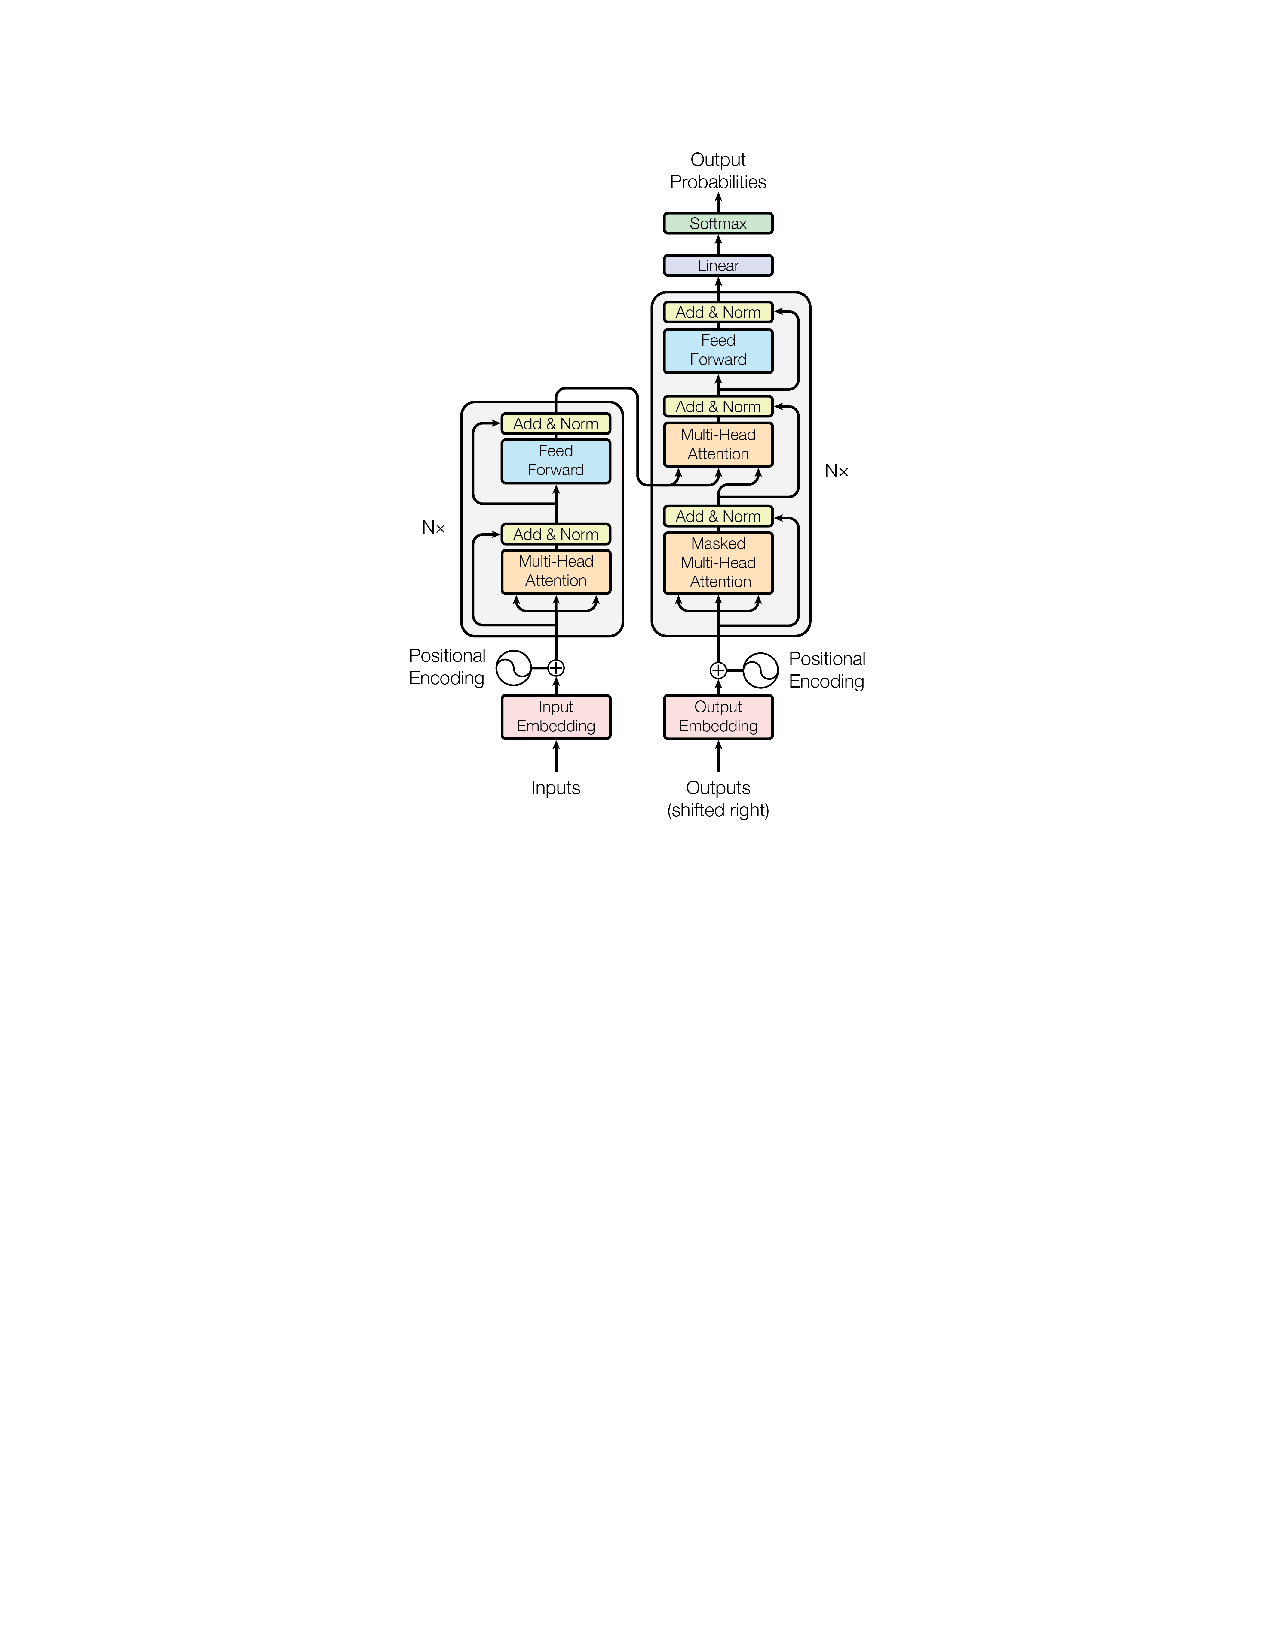
\includegraphics[width=0.55\textwidth]{figures/transformer.pdf}
\bicaption{Transformer模型架构\cite{vaswani2017attention}}{The Transformer - model architecture\cite{vaswani2017attention}}
\label{fig:transformer}
\end{figure}

\begin{figure}[!t]
\centering
\subcaptionbox{HOG + SVM\label{fig:meme:yes}}
    {
\includegraphics[width=0.25\linewidth]{figures/yes.jpg}}
\subcaptionbox{Neural Network\label{fig:meme:no}}
    {
\includegraphics[width=0.25\linewidth]{figures/no.jpg}}
\bicaption{多个分图的示例}{Multiple Sub-Figures}
\label{fig:meme}
\end{figure}

若图或表中有附注,采用英文小写字母顺序编号,附注写在图或表的下方。
国外的期刊习惯将图表的标题和说明文字写成一段,需要改写为标题只含图表的名称,其他说明文字以注释方式写在图表下方,或者写在正文中。

如果一个图由两个或两个以上分图组成时,各分图分别以 (a)、(b)、(c)...... 作为图序,并须有分图标题。
推荐使用 \texttt{subcaption} 宏包来处理, 比如图~\ref{fig:meme:yes} 和图~\ref{fig:meme:no}。


\bisection{表}{Tables}

表应具有自明性。为使表格简洁易读,尽可能采用三线表,如表~\ref{tab:datasets}。
三条线可以使用 \texttt{booktabs} 宏包提供的命令生成。

\begin{table}[htbp]
\small
\centering
\bicaption{数据集概览}{Summary of Datasets}
\begin{tabular}{lcccccc}
\toprule
数据集 & 样本数量 & 记录数量 & 特征数量 & 平均记录数量 & 类别数 & $p/r$\\
\midrule
PPMI & 683 & 15798 & 212 & 23.1303 & 2 & 9/1 \\
PS & 68 & 1208 & 26 & 17.7647 & 2 & 1.5/1 \\
OD & 115 & 20560 & 5 & 178.7826 & 2 & 1/36 \\
\bottomrule
\end{tabular}
\label{tab:datasets}
\end{table}


\bisection{算法}{Algorithms}

算法环境可以使用 \texttt{algorithms} 宏包。

\begin{algorithm}[htbp]
\caption{算法示例}
\label{alg:cram_mult}
\begin{algorithmic}[1]
\State $i \gets 10$
\If{$i\geq 5$} 
    \State $i \gets i-1$
\Else
    \If{$i\leq 3$}
        \State $i \gets i+2$
    \EndIf
\EndIf
\end{algorithmic}
\end{algorithm}
\include{chapters/chapter-4}
\include{chapters/chapter-5}

\chapter*{结\quad\quad 论} % Unnumbered chapter* in backmatter
\addcontentsline{toc}{chapter}{结\quad 论} % Manually add to TOC
\label{chap:conclusion}

结论是理论分析和实验结果的逻辑发展,是整篇论文的归宿。结论是在理论分析、试验结果的基础上,经过分析、推理、判断、归纳的过程而形成的总观点。结论必须完整、准确、鲜明、并突出与前人不同的新见解。

书写格式说明:

标题“结论”选用模板中的样式所定义的“标题1”,再居中;或者手动设置成字体:黑体,居中,字号:小三,1.5倍行距,段后11磅,段前为0。

结论正文选用模板中的样式所定义的“正文”,每段落首行缩进2字;或者手动设置成每段落首行缩进2字,字体:宋体,字号:小四,行距:多倍行距 1.25,间距:前段、后段均为0行。


%-----------------------------------------------------------------------------------------------------------------------

\bibliography{references/paper-manual}

%-----------------------------------------------------------------------------------------------------------------------
\appendix
% appendix.tex

\chapter{附录内容名称} % Appendix chapters are numbered A, B, ...
\label{app:example}

这里是附录A的正文内容。

\section{附录中的节}
% Appendix sections are numbered A.1, A.2, ...
可以使用图、表等。 Equation:
\begin{equation}
    E = mc^2
\end{equation}


%-----------------------------------------------------------------------------------------------------------------------
%\backmatter
% achievements/achievements.tex - Minimal Test Achievements
\chapter*{攻读硕士学位期间发表学术论文情况}
\addcontentsline{toc}{chapter}{攻读硕士学位期间发表学术论文情况}

%\noindent
仅列出硕士生攻读硕士学位期间发表与学位论文有关的学术论文,并注明属于学位论文内容的部分(章节),所有作者及其顺序、所发表的刊物名称(包括主办单位、是否被SCI、EI检索期刊)、时间、期号与页码。其他时间或与学位论文内容(章节)无关的论文不得列出。

书写格式说明:

标题“攻读硕士学位期间发表学术论文情况”选用模板中的样式所定义的“标题1”,再居中;或者手动设置成字体:黑体,居中,字号:小三,1.5倍行距,段后11磅,段前为0。

在学研究成果正文选用模板中的样式所定义的“正文”,每段落首行缩进2字;或者手动设置成每段落首行缩进2字,字体:宋体,字号:小四,行距:多倍行距 1.25,间距:前段、后段均为0行。

```
% acknowledgement/acknowledgement.tex - Minimal Test Acknowledgement
\chapter*{致\quad 谢} % Unnumbered chapter* in backmatter
\addcontentsline{toc}{chapter}{致\quad 谢} % Manually add to TOC

%\noindent
学位论文中不得书写与论文工作无关的人和事,对导师的致谢要实事求是。

对一同工作的同志在本研究所做的贡献应于论文中做明确的说明并表示谢意。

这部分内容不可省略。

书写格式说明:

标题“致谢”选用模板中的样式所定义的“标题1”,再居中;或者手动设置成字体:黑体,居中,字号:小三,1.5倍行距,段后11磅,段前为0。

致谢正文选用模板中的样式所定义的“正文”,每段落首行缩进2字;或者手动设置成每段落首行缩进2字,字体:宋体,字号:小四,行距:多倍行距 1.25,间距:前段、后段均为0行。



\cleardoublepage
\phantomsection  % 为超链接添加锚点
\addcontentsline{toc}{chapter}{大连大学学位论文版权使用授权书}  % 添加到一级目录
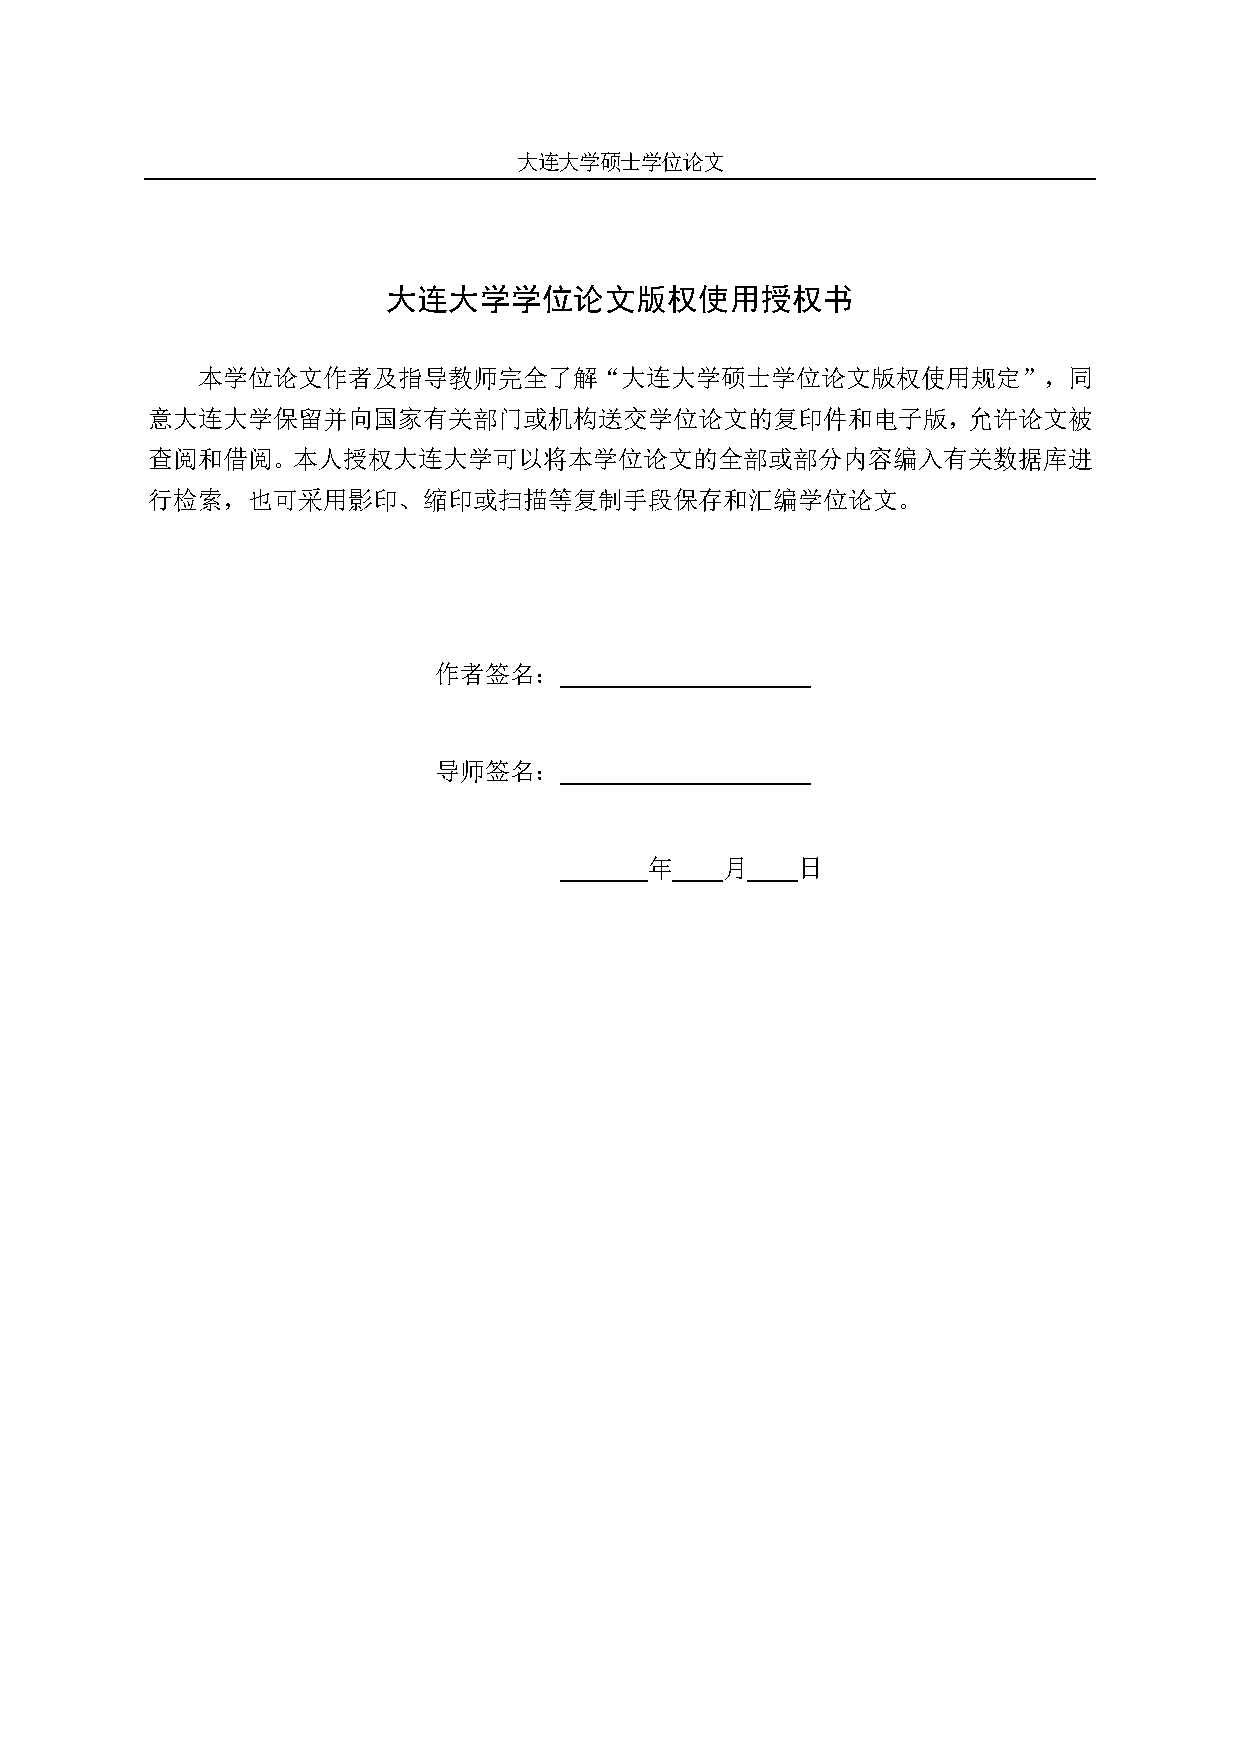
\includepdf[pages=-]{copyright.pdf}
%-----------------------------------------------------------------------------------------------------------------------
\end{document}
